\chapter{弱いPCP定理}

この章はPCP検証者における「少ないクエリ回数」という要件がなぜ達成できるかについて説明することを目的とする.
そのため, まずはPCP定理の要件であるランダムビットの短さはひとまず無視した以下の形の「弱いPCP定理」を証明する: 任意の$\NP$に属する判定問題が$O(1)$クエリかつ$\poly(n)$ビットのランダムネスを用いて確率的に検証可能である.

\section{局所的な検証はなぜ可能なのか?}
PCP検証者は, オラクルアクセスとして与えられた証明のうち, 定数文字のみを見てその証明がちゃんと証明たりうるかを判定しなければならない.
ここでは, 定数個の文字のみを見るという性質を検証者の局所性と呼ぶことにする.

一般的な感覚として, ある主張が成り立つことを示す証明を検証する際, \emph{冗長に表現で記述しない限り}その証明を全て読み込まなければ検証できないと思われる (全ての文字に本質的な意味があるならば全てを確認しなければならないはずであろう).
では逆に, 証明を冗長に表現することで局所的な検証を可能にすることはできるだろうか?

\subsection{線形方程式に対する局所的な検証(1/2)}
興味深いことに, 非常に冗長性が大きい記述で証明が与えられたならば局所検証が可能であることを, 線形方程式の検証を例に説明する.

\begin{definition}{線形方程式}{linear-equation}
有限体$\F$上の行列$M\in\F^{m\times n}$とベクトル$z\in\F^m$に対して
\begin{align*}
  My = z
\end{align*}
を満たす$y\in\F^n$が存在するかどうかを判定する問題を$\LinEq$とする.
ここで$\abs{\F}=q$は$m,n$とは独立な定数であるとする (従って有限体上の演算は$O(1)$時間で計算できると仮定する).
\end{definition}

愚直な検証者として$y\in\F^n$を証拠として受け取り, $My=z$を確認することで検証を行うことを考える (実際の計算機では全てを二進文字列で表現するため, $\F$の元は$\ceil{\log_2\abs{\F}}=O(1)$ビットで表現されている).
明らかにこの検証者は$My$を計算するために$y$の全ての成分 (すなわち$O(n)$ビット) を読み込む必要があるため, オラクルアクセスの回数が大きくなり局所性を持たない.
もちろん, この判定問題は標準的な線型方程式の解の存在性判定であるため, 掃き出し法を用いれば証拠へのオラクルアクセスなしでも多項式時間で解ける.
しかしここではあえて, 局所的な検証の構成例を与えるという目的で取り扱う.

重要な性質として, 二つのベクトル$a,b\in\F^n$に対する次の性質を考える (証明は\cref{exer:random-inner-product}):
\begin{align}
  \Pr_{r\sim \F^n} \qty[ r^\top a \ne r^\top b ] = \begin{cases}
    0 & \text{if } a=b \\
    1-\frac{1}{q} & \text{if } a\ne b.
  \end{cases} \label{eq:linear-equation-property}
\end{align}
さて, \cref{eq:linear-equation-property}の性質を用いると一様ランダムな$r\sim\F^n$に対して
\begin{align}
  r^\top M y = r^\top z \label{eq:random-inner-product}
\end{align}
かどうかを確認することで, $My=z$かどうかを確率的に検証できる.
実際, $My=z$ならば確率$1$で検証者は受理し,
$My\ne z$ならば確率$1-1/q$で検証者は拒否する (何度も繰り返せばこの拒否率を任意に$1$に近い定数まで近づけることができる).
ベクトル$z$は入力として与えられているため\cref{eq:random-inner-product}の右辺は$O(n)$時間で計算できる.
一方で, ベクトル$y$は証拠として与えられるため, $r^\top M y$の計算は愚直に考えると$O(mn)$時間かかる上に$y$の全ての成分を読み込む必要がある.
ところが, 全てのベクトル$w\in \F^n$に対して$y^\top w\in\F$を連結して得られる長さ$q^n$の文字列$(y^\top w)_{w\in \F^n}$を証拠$\pi$として与えることにより,
自身で$r^\top M$を計算した後に $r^\top M y = y^\top (M^\top r)$の値を\emph{一文字の証拠の読み込み}で計算できるのである.

\begin{exercise}{ランダムなベクトルとの内積}{random-inner-product}
  \cref{eq:linear-equation-property}を証明せよ.
\end{exercise}

このように, ベクトル$y\in\F^n$を, それを係数とする線形関数$w\mapsto y^\top w$の\emph{真理値表(全ての点での評価値を並べた文字列)として冗長に表現する}ことで, 証拠の読み込み回数を定数に抑えるというのが基本的なアイデアである.
このように文字列を冗長に表現する手法を総称して\emph{誤り訂正符号}という.
本講義では, \emph{アダマール符号}と呼ばれる以下の誤り訂正符号を用いる:
\begin{definition}{アダマール符号}{Hadamard-code}
  有限体$\F$上のベクトル$y\in\F^n$に対して, 長さ$q^n$の文字列
  \begin{align*}
    \Had_n(y) = (y^\top w)_{w\in \F^n}
  \end{align*}
  を考える.
  集合$\Had_n = \qty{ \Had_n(y) \colon y\in \F^n }$を\emph{アダマール符号}といい,
  その元を\emph{アダマール符号の符号語}という.
  また, $\Had_n(y)$を\emph{$y$をアダマール符号で符号化した文字列}という.

  なお, 次元$n$が明らかなときは省略して$\Had(y)$などと表す.
\end{definition}

\begin{remark}{}{string-vector-function}
  本講義では文字列, ベクトル, 関数をしばし同一視する.
  すなわち, ベクトル$x\in\F^n$を単に文字列と呼ぶこともあり,
  または関数$x\colon [n]\to\F$とみなすこともある.
  例えば$y\in\F^n$をアダマール符号で符号化した文字列$\Had(y)$は, 長さ$q^n$の文字列とみなすこともあれば,
  関数$\Had(y)\colon \F^n\to\F$とみなすこともある.

  これは, アダマール符号の解析の過程では$\Had(y)$を関数とみなして扱う方が都合が良いものの,
  PCP定理の証明の過程では$\Had(y)$を文字列として扱い, 証明$\pi$として与えることになるからである.
\end{remark}

素朴な証拠$y$をアダマール符号で符号化したものを証明として扱うというアイデアを素朴に実装すると, $\LinEq$に対する局所的な検証(の候補)として以下の検証者を考えることができる:
\begin{algo}{}{local-verification-LinEq?}
  \begin{enumerate}
  \item 入力として$M,z$を受け取り, 証拠として$\pi \in \F^{q^n}$へのオラクルアクセスを受け取る.
  \item 一様ランダムな$r\sim\F^m$を選択し, $r^\top M$と$r^\top z$を計算する.
  \item 証拠$\pi\colon \F^{q^n}$を関数$\pi\colon \F^n\to \F$として解釈し, オラクルアクセスを用いて$a=\pi(M^\top r)$を求める.
  \item $a=r^\top z$ならば$1$を出力し, そうでなければ$0$を出力する.
  \end{enumerate}
\end{algo}

上記の検証者はPCP検証者の性質を持つだろうか?
まず, $(M,z)$がYesインスタンスであるとき, ある$y\in\F^n$が存在して$My=z$が成り立つ.
このとき, $\pi=\Had(y)\colon\F^n\to\F$とすると, $\pi(M^\top r)=y^\top (M^\top r)=r^\top (My)=r^\top z$となるため, 検証者は確率$1$で受理する.

一方で$(M,z)$がNoインスタンスであるときに検証者が拒否する確率はどうなるだろうか?
PCP検証者であることを示す(cf. \cref{def:PCP})には, 任意の$\pi\in\F^n\to\F$に対して拒否確率は少なくとも$1/3$以上でなければならない.
これは示せるのであろうか?
証明$\pi$がアダマール符号の符号語である(すなわち, ある$y\in\F^n$に対して$\pi = \Had(y)$と表せる)場合は, \cref{eq:random-inner-product}の性質および$(M,z)$がNoインスタンスであることから$My\ne z$より, 少なくとも確率$1-1/q$で検証者は拒否する.
しかしながら, 一般の$\pi\in\F^n\to\F$はこのような線形関数として表現できるとは限らず, そのような$\pi$に対しても拒否しなければならない.

\subsection{線形性テスト}
与えられた$(M,z)$がNoインスタンスであるときに任意の$\pi\in\F^{q^n}$を定数確率で拒否するために,
\cref{alg:local-verification-LinEq?}を以下のように修正する:
証拠$\pi$がアダマール符号の符号語ならば, \cref{alg:local-verification-LinEq?}のステップ2-4を実行し, そうでないならば$0$を出力する.
ここで新たに一つの問題が生じる: どのようにして$\pi$の線形性を局所検証すればよいだろうか?

一般にオラクルアクセスで与えられた関数$\pi\colon\F^n\to\F$が線形関数かどうかを厳密に確認するには,
\begin{align}
  \forall x,y\in\F^n,\quad \pi(x+y)=\pi(x)+\pi(y) \label{eq:linearity-test-all-points}
\end{align}
が成り立つかどうかを確認する必要があり, $q^n$回のオラクルアクセスが必要となってしまう.

そこで, 「線形関数であるかどうか」ではなく「線形関数に近いかどうか」を局所検証することを考える.
\begin{definition}{関数同士の近さ}{distance-between-functions}
  二つの関数$f,g\colon A \to B$に対して$\dist(f,g)$を
  \begin{align*}
    \dist(f,g) =\Pr_{a\sim A} \qty[ f(a) \ne g(a) ]
  \end{align*}
  と定義し, $\dist(f,g)\le\delta$を満たすとき, $f$は$g$に\emph{$\delta$-近い}($\delta$-close)という.
  
  また, 関数クラス$\calF\subseteq \qty{ g\colon A\to B }$および関数$f\colon A\to B$に対して
  \begin{align*}
    \dist(f,\calF) = \min_{g\in\calF} \dist(f,g)
  \end{align*}
  と定義し, $\delta(f,\calF)\le \delta$であるとき, $f$は$\calF$に$\delta$-近いという.
\end{definition}

関数$f\colon A\to B$をベクトル$f\in B^A$と同一視すると, $\dist(f,g)$はベクトル$f,g$間の正規化されたハミング距離($\ell_0$ノルム)に一致する.

線形関数全体$\Had\subseteq\qty{\F^n\to\F}$を考える (\cref{def:Hadamard-code}).
オラクルアクセスとして与えられた関数$\pi\colon \F^n\to\F$が$\Had$に近いかどうかを検証する局所検証者が構成できる \citet{BLR93}.

\begin{theorem}{線形性テスト}{linearity-test}
  以下を満たす乱択多項式時間オラクルアルゴリズム$A^\pi(1^n)$が存在する\footnote{アルゴリズム$A$は$1^n$を入力として与えられているため, 多項式時間であることは計算量が$\poly(n)$で抑えられることを意味する.}:
  関数$\pi\colon \F^n\to\F$がオラクルアクセスとして与えられたとき,
  \begin{itemize}
    \item $\pi\in \Had$ならば$A^\pi(1^n)$は確率$1$で受理する.
    \item $\dist(\pi,\Had)\ge 0.01$ならば$A^\pi(1^n)$は確率$0.99$で拒否する.
  \end{itemize}
\end{theorem}

\begin{remark}{符号の局所検査性}{locally-testable-code}
  \cref{thm:linearity-test}はアダマール符号$\Had\subseteq\F^{q^n}$は, オラクルアクセスとして与えられた文字列$\pi\in\F^{q^n}$がその符号語か, もしくは$\Had$から遠いかどうかを, $O(1)$回のオラクルアクセスで確立的に判定できることを意味する.
  このような性質を持つ誤り訂正符号を\emph{局所検査可能符号} (locally testable code)という.
\end{remark}
\begin{proof}
  アルゴリズム$A^\pi$は非常に単純で, 線形関数であることの特徴づけ\cref{eq:linearity-test-all-points}をランダムな点で確認するというものである.
  具体的には以下で与えられる:
  \begin{algo}{}{linearity-test}
    \begin{enumerate}
      \item オラクルアクセスとして関数$\pi\colon \F^n\to\F$を受け取り, 入力として$1^n$を受け取る.
      \item 一様ランダムに$x,y\sim\F^n$を選び, $\pi(x+y)\ne \pi(x)+\pi(y)$が成り立つならば拒否する.
      \item 十分大きな定数$K\in\Nat$に対し, ステップ2を$K$回繰り返す. この繰り返しの中で一度も拒否しなければ, 受理する.
    \end{enumerate}
  \end{algo}

  実際, $\pi\in\Had$ならば\cref{eq:linearity-test-all-points}が成り立つため, $A^\pi(1^n)$は確率$1$で受理する.
  一方で, $\dist(\pi,\Had)\ge 0.01$であるときに拒否確率を下から抑えたい.
  これは以下の主張から従う:

  \begin{claim}{線形性テストの拒否確率}{linearity-test-rejection-probability}
    任意の関数$\pi\colon \F^n\to\F$に対して
    \begin{align*}
      \Pr_{x,y\sim\F^n}\qty[ \pi(x+y) \ne \pi(x)+\pi(y) ] \ge \frac{1}{6}\cdot \dist(\pi,\Had).
    \end{align*}  
  \end{claim}

  \cref{claim:linearity-test-rejection-probability}は後で証明する.
  仮定より$\dist(\pi,\Had)\ge \delta:=0.01$なので,
  ステップ3の定数$K$を十分大きくすることによって, \cref{alg:linearity-test}の拒否確率を$0.99$より大きくすることができる.
  \end{proof}

  次に\cref{claim:linearity-test-rejection-probability}を示す.
  実際にはより一般的な次の補題を証明する.
  \begin{lemma}{準同型性テスト}{homomorphism-test}
    有限アーベル群$G,H$に対し, 写像$f\colon G\to H$が準同型であるとは, 任意の$x,y\in G$に対して$f(x+y)=f(x)+f(y)$が成り立つことをいい, $G$から$H$への準同型な写像の全体を$\calH$と表す.
    このとき, 任意の関数$f\colon G\to H$に対して
    \begin{align*}
      \Pr_{x,y\sim G}\qty[ f(x+y)\ne f(x)+f(y) ] \ge \frac{1}{12}\cdot \dist(f,\calH).
    \end{align*}
  \end{lemma}
  \begin{proof}
    記号の簡単のため, $\rho_f:=\Pr_{x,y\sim G}\qty[ f(x+y)\ne f(x)+f(y) ]$と表す.
    また, 各$y\in G$に対し, 写像$v_y\colon G\to H$を$v_y(x)=f(x+y)-f(y)$とし, $v\colon G\to H$を
    \begin{align*}
      v(x) = \mathrm{argmax}_{a \in H} \qty{ \Pr_{y\sim G}\qty[ v_y(x)=a ] }
    \end{align*}
    で定める (タイが存在する場合は任意).
    すなわち, $v(x)$は$(v_y(x))_{y\in G}$の中での多数決, すなわち最も出現頻度の高い値として定める.
    証明は以下の三つの主張を組み合わせることによって得られる.
    
    \begin{claim}{}{claim1}
      $\dist(f,v) \le 2\rho_f$が成り立つ.
    \end{claim}
    \begin{proof}
      定義より$\rho_f = \Pr_{x,y}[f(x) + f(y) \ne f(x+y)] = \Pr_{x,y} [ f(x) \ne v_y(x)]$ である.
      また, $v(x)\ne h\Rightarrow \Pr_y[v_y(x)= h]\le 1/2 \iff \Pr_y[v_y(x)\ne h]\ge 1/2$が成り立つ.
      実際, $(v_y(x))_{y\in G}$の中で多数決をとったときに$h$が選ばれなかったということは, 過半数に至らなかったことを意味するからである.
      特に, $h=f(x)$とすると, $\mathbf{1}_{v(x)\ne f(x)} \le 2\Pr_y[v_y(x)\ne f(x)]$.
      両辺の$x\sim G$に関する期待値をとると
      \begin{align*}
        \dist(f,v) = \Pr_x[v(x)\ne f(x)] \le 2\Pr_{x,y}[v_y(x)\ne f(x)] =2\rho_f.
      \end{align*}
      となり主張を得る.
    \end{proof}
    
    \begin{claim}{}{claim2}
      $\rho_f<1/6$ ならば, 全ての$x\in G$に対して$\Pr_y[v_y(x)= v(x)] > 2/3$.
    \end{claim}
    \begin{proof}
      任意に $x\in G$ を固定し, 確率変数$\Phi$を, 一様ランダムに$y\sim G$を選び $\Phi=v_y(x)$ として定める. 我々の目標は, ある$a\in H$に対して$\Pr[\Phi=a]>2/3$ が成り立つことを示すことである.
      $\Phi_1,\Phi_2$を$\Phi$の独立なコピーとする (固定する$x$は同一). $\Phi$がある値をとる傾向にあることを示すために, まずは $\Phi_1=\Phi_2$ が成り立つ確率が大きいことを示す.
      \begin{align*}
      \Pr[\Phi_1 = \Phi_2] &= \Pr_{y_1,y_2\sim G}[ v_{y_1}(x) = v_{y_2}(x) ] \\
      &= \Pr_{y_1,y_2}[ f(x+y_1) - f(y_1) = f(x+y_2) - f(y_2) ] \\
      &= \Pr_{y_1,y_2}[ f(x+y_1)-f(x+y_2) = f(y_1)-f(y_2) ] \\
      &\ge 1-2\rho_f \\
      &> 2/3.
      \end{align*}    
      最初の不等式では, $\Pr_{y_1,y_2}[f(x+y_1)-f(x+y_2) \ne f(y_1-y_2)]\le \rho_f$ および $\Pr_{y_1,y_2}[f(y_1)-f(y_2)\ne f(y_1-y_2)]\le \rho_f$ を用いた.    
      ここで, $2/3<\Pr[\Phi_1=\Phi_2]=\sum_{a\in H}\Pr[\Phi=a]^2 \le \max_a\Pr[\Phi=a]\cdot \sum_{a\in H}\Pr[\Phi=a] = \max_a\Pr[\Phi=a]$ より主張を得る.
    \end{proof}

    \begin{claim}{}{claim3}
      全ての $x\in G$ に対して $\Pr_y[v_y(x)=v(x)]>2/3$ が成り立つならば, $v\in \calH$, すなわち$h$は準同型である.
    \end{claim}
    \begin{proof}
      全ての$x,y\in G$に対して$f(x)+f(y)=f(x+y)$が成り立つことを示せばよい. 任意に$x,y\in G$を固定する.
      一様ランダムな$z\sim G$ を選ぶ. このとき, 仮定より
      \begin{itemize}
        \item $\Pr_z[v_z(x)\ne v(x)]<1/3$,
        \item $\Pr_z[v_{z-y}(y)\ne v(y)]<1/3$,
        \item $\Pr_z[v_{z-y}(x+y)\ne v(x+y)]<1/3$
      \end{itemize}
      従って, ユニオンバウンドより, 任意の $x,y\in G$ に対してある$z\in G$が存在して次の三つが同時に成り立つ:
      \begin{itemize}
        \item $v(x)=v_z(x)=f(x+z)-f(z)$,
        \item $v(y)=v_{z-y}(y)=f(z)-f(z-y)$,
        \item $v(x+y)=v_{z-y}(x+y)=f(x+z)-f(z-y)$
      \end{itemize}
      これらの等式から
      \begin{align*}
        v(x)+v(y)-v(x+y) = f(x+z)-f(z-y) - (f(x+z)-f(z-y)) = 0.
      \end{align*}
      より主張を得る.
    \end{proof}
    最後に\cref{lem:homomorphism-test}の証明を完成させる.
    $\rho_f<1/6$ならば, \cref{claim:claim2,claim:claim3}より, $v\in\calH$である.
    さらに\cref{claim:claim1}より,
    \begin{align*}
      \rho_f \ge \frac{\dist(f,v)}{2} \ge \frac{\dist(f,\calH)}{2}
    \end{align*}
    である. 一方, そうでなければ$\rho_f\ge 1/6 \ge \dist(f,\calH)/6$である.
    いずれにせよ, $\rho_f\ge \dist(f,\calH)/6$が成り立つ.
  \end{proof}
  
  以上より, 与えられた$\pi$が$\Had$に近いかどうかを局所検証できることを示した.
  では, 仮に$\pi$が$\Had$に近いとし,
  最も近い線形関数を$f\in\Had$としよう.
  このような$f\in\Had$は一意である (\cref{exer:uniqueness-of-nearest-linear-function}).
  このとき, 99\%の$x\sim\F^n$に対して$\pi(x)=f(x)$が成り立つ.
  一方で\cref{alg:local-verification-LinEq?}では$f(M^\top r)$を計算する必要があり,
  一般に$r\sim\F^m$に対して$M^\top r$の分布は一様ランダムとは限らない.
  そこで, 任意の点$x\in\F^n$に対して$f(x)$を計算することが必要であり,
  次の補題はこれが可能であることを示している.

  \begin{lemma}{最も近い線形関数の任意点での評価}{nearest-linear-function-evaluation}
    関数$\pi\colon\F^n\to\F$が$\dist(\pi,\Had)\le \epsilon$を満たすとし,
    $\pi$に最も近い線形関数を$f\in\Had$とする.
    このとき, 任意の$x\in\F^n$を入力として受け取り, $\pi$への2回のオラクルアクセスを用いて$O(n)$時間で$f(x)$を確率$1-2\epsilon$で出力する乱択オラクルアルゴリズム$A^\pi(x)$が存在する.
  \end{lemma}
  \begin{proof}
    入力として与えられた$x\in\F^n$に対して, $A^\pi(x)$はランダムな$r\sim\F^n$を選び, $\pi(x+r)-\pi(r)$を出力する.
    明らかに時間計算量は$O(n)$であり, $\Pr_r[\pi(x+r)\ne f(x+r)], \Pr_r[\pi(r)\ne f(r)]$はそれぞれ$\epsilon$以下である.
    従って, 確率$1-2\epsilon$で出力値は$\pi(x+r)-\pi(r)=f(x+r)-f(r)=f(x)$となる.
  \end{proof}
  
  \begin{exercise}{最も近い線形関数の唯一性}{uniqueness-of-nearest-linear-function}
  関数$\pi\colon\F^n\to \F$が$\dist(\pi,\Had) \le 0.01$を満たすとき,
  $\dist(\pi,f)\le 0.01$を満たす$f\in\Had$は唯一存在することを示せ.
  \end{exercise}


\subsection{線形方程式の局所的な検証(2/2)}
ここまでの議論を用いて$\LinEq$に対する局所的な検証者を構成する.
\begin{algo}{}{local-verification-LinEq}
  \begin{enumerate}
    \item 入力として$M,z$を受け取り, 証拠として$\pi \in \F^{q^n}$へのオラクルアクセスを受け取る.
    \item \cref{thm:linearity-test}のアルゴリズムを$\pi$をオラクルとして実行し, $\dist(\pi,\Had)\ge 0.01$ならば拒否して終了する.
    \item 一様ランダムな$r\sim\F^m$を選択し, $r^\top M$と$r^\top z$を計算する.
    \item \cref{lem:nearest-linear-function-evaluation}のアルゴリズムを$M^\top r$を入力, $\pi$をオラクルとして実行し, その出力を$a$とする.
    \item $a\ne r^\top z$ならば拒否する.
    \item ステップ3-5を3回繰り返し, 一度も拒否しなければ受理して終了する.
  \end{enumerate}
\end{algo}
\cref{alg:local-verification-LinEq?}の検証者と比較すると,
まず, 証拠として与えられた関数$\pi$が線形関数であることを検証するためのステップが追加されている.
また, ステップ4では$\pi(M^\top r)$の代わりに\cref{lem:nearest-linear-function-evaluation}のアルゴリズムが用いられている.
これまでの議論から, \cref{alg:local-verification-LinEq}は$\LinEq$に対する局所的な検証者であることがわかる.
ステップ6は単に成功確率を増幅させるための繰り返しである.

\begin{theorem}{線形方程式の局所的な検証}{local-verification-LinEq}
  \cref{alg:local-verification-LinEq}の検証者を$V^\pi(M,z)$とする.
  このとき, 任意の$M\in\F^{m\times n},z\in\F^m$に対して以下が成り立つ:
  \begin{itemize}
    \item $V^\pi(M,z)$の$\pi$へのオラクルアクセスの回数は$O(1)$である.
    \item $My=z$を満たす$y\in\F^n$が存在するならば, $\pi=\Had(y)$としたとき, $V^\pi(M,z)$は確率$1$で受理する.
    \item $My=z$を満たす$y\in\F^n$が存在しないならば, 任意の$\pi\colon\F^n\to\F$に対して$V^\pi(M,z)$は確率$2/3$で拒否する.
  \end{itemize}
\end{theorem}
\begin{proof}
  オラクルアクセスの回数は明らかに$O(1)$である.
  また, $My=z$を満たす$y\in\F^n$が存在するならば, $\pi=\Had(y)$としたとき, 確率$1$で受理する.
  一方, $My=z$を満たす$y\in\F^n$が存在しないときに検証者が拒否する確率を考える.
  オラクル$\pi$に関して以下の二つのケースを考える:

  \paragraph*{ケース1: $\pi$が線形関数に$0.01$-近いとき.}
  このとき, $V^\pi(M,z)$がステップ5で拒否する確率を評価する.
  オラクル$\pi$に最も近い線形関数を$f\colon \F^n\to\F$とする.
  このとき, \cref{lem:nearest-linear-function-evaluation} (入力を$M^\top r$, $\epsilon=0.01$とする)より, ステップ4で計算される$a$は, 確率$1-2\epsilon=0.98$で$f(M^\top r)$と等しい.
  ここで, 線形関数$f$が$f(x)=x^\top y$と表せるとすると, 拒否確率は
  \begin{align*}
    \Pr\qty[ a \ne r^\top z ] &\ge \Pr_{r}\qty[ a\ne r^\top z \mid a = f(M^\top r) ] \cdot \Pr_{r}\qty[ a = f(M^\top r) ] \\
    &\ge \Pr_{r}\qty[ r^\top M y \ne r^\top z ]\cdot 0.98 \\
    &\ge \qty(1-\frac{1}{q}) \cdot 0.98 & & \because \text{\cref{eq:random-inner-product}および$My\ne z$} \\
    &\ge 0.4 & & \because\text{$q\ge 2$}
  \end{align*}
  を満たす.
  これを4回繰り返すため, 拒否確率は少なくとも$1-(1-0.4)^3\ge \frac{2}{3}$を満たす.
  

  \paragraph*{ケース2: $\pi$が線形関数に$0.01$-遠いとき.}
  このとき, \cref{thm:linearity-test}より, $V^\pi(M,z)$はステップ2において少なくとも確率$0.99$で拒否する.
  
  従って, どちらのケースでも, $V^\pi(M,z)$は少なくとも確率$2/3$で拒否する.
  
\end{proof}

ここまでの議論を用いると以下のように, オラクルを用いて線形方程式の解を効率的に検証する検証者が構成できる.

  \begin{lemma}{線型方程式の解の検証}{linear-equation-solution-verification}
    以下を満たす定数$q=O(1)$と乱択$O(mn)$時間オラクルアルゴリズム$V^{\pi}(M,z)$が存在する:
    入力として$M\in\F^{m\times n},z\in\F^m$を受け取り, オラクルとして$\pi\colon\F^n\to\F$へのオラクルアクセスを受け取り, これらのオラクルに対して合計で高々$q$回のオラクルアクセスを行う. 任意のオラクル$\pi$に対し以下が成り立つ:
    \begin{itemize}
      \item あるベクトル$y\in\F^n$に対して$\pi=\Had_n(y)$であるならば, $V^{\pi}(M,z)$は確率$1$で受理する.
      \item $My=z$を満たす全てのベクトル$y\in\F^n$に対して$\dist(\pi,\Had_n(y))\ge 0.01$ならば, $V^{\pi}(M,z)$は確率$0.99$で拒否する.
    \end{itemize}
  \end{lemma}

  \begin{figure}[htbp]
    \centering
    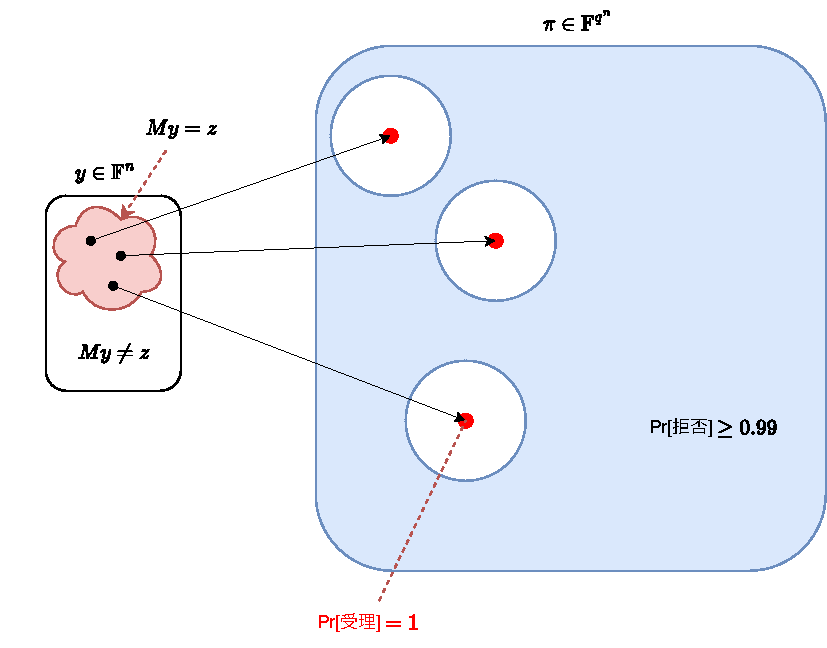
\includegraphics[width=0.8\textwidth]{images/linear_verification.pdf}
    \caption{\cref{lem:linear-equation-solution-verification}の検証者のイメージ. $My=z$を満たす$y$に対し$\Had_n(y)$がオラクルとして与えられたときは常に受理する. 一方, そのような全ての$\Had_n(y)$から離れた$\pi$は高確率で拒否する.}
  \end{figure}
  
  \begin{exercise}{線型方程式の解の検証}{linear-equation-solution-verification}
    \cref{lem:linear-equation-solution-verification}を証明せよ (ヒント: \cref{eq:random-inner-product,lem:nearest-linear-function-evaluation}を用いる).
  \end{exercise}

\section{弱いPCP定理とその証明}
\cref{thm:local-verification-LinEq}のアイデアを拡張してPCP定理を証明するには何が必要だろうか?
\begin{itemize}
  \item まず, $\LinEq$は実際には多項式時間で解ける判定問題であるが, 実際には何かしらのNP完全な判定問題に対して\cref{thm:local-verification-LinEq}のような検証者を構成しなければならない.  
  \item 次に, \cref{thm:local-verification-LinEq}の検証者$V^\pi(M,z)$は, ランダムに$r,r'\sim\F^n$を選ぶ時点で$\Omega(n)$ビットのランダムネスを必要とする. 実際, 証拠として与えられた関数$\pi$を文字列として表現するとその長さは$q^n$に比例するため, その文字列のランダムなインデックスを指定しようとすると必然的に$\Omega(n)$ビットのランダムネスが必要である. そこで証明$\pi$の長さを指数的な長さ$2^{\Theta(n)}$から多項式$n^{O(1)}$に抑える必要がある (このとき, インデックスの指定に必要なビット数は$O(\log n)$で抑えられる).
\end{itemize}

本節では前者の問題を解決し, 以下の弱いPCP定理を証明する.
\begin{theorem}{弱いPCP定理}{weak-PCP-theorem}
  ある$r(n)=\poly(n),q(n)=O(1)$に対して, $\NP \subseteq \PCP(r,q)$が成り立つ.
\end{theorem}

我々の最終的な目標であるPCP定理(\cref{thm:PCPtheorem})では, PCP検証者のランダムビットの長さが$r(n)=O(\log n)$であることを要求しているため, $r(n)$に関しては\cref{thm:weak-PCP-theorem}は指数的に大きい値になってしまっているが, 読み込む証明の文字数は$n$に依存しない定数で抑えられるという点では同一である.
なお, \cref{thm:weak-PCP-theorem}の証明のアイデアは後に\cref{thm:PCPtheorem}の証明でも用いられる.

\subsection{方針}
  \cref{thm:ThreeQuadEQ-NP-complete}で定義した問題$\QuadEQ$に対してPCP検証者を構成すればよい.
  ここではより一般的に, ある$r=O(1),q=\poly(n)$に対して$\QuadEQ\in\PCP(r,q)$を示す.
  $\QuadEQ$のインスタンスは
  \begin{align*}
    &f_1(x_1,\dots,x_n) = 0,\\
    &\quad\vdots\\
    &f_m(x_1,\dots,x_n) = 0
  \end{align*}
  という$m$個の$\F_2$上の二次連立方程式からなる.
  
  ここで$y_{i,j}=x_ix_j$としてこれらを並べたベクトル$y\in\F_2^{n^2}$を考える (ここでは$(i,j)$を$[n^2]$の元として扱う).
  各$k\in[m]$と$i,j\in[n]$に対し,
  \begin{align}
    &M_{k,(i,j)} = \begin{cases}
      1 & \text{if $f_k(x_1,\dots,x_n)$が項$x_i x_j$を含む},\\
      0 & \text{otherwise},
    \end{cases} \label{eq:M-matrix}\\
    &b_k = f_k(0) \label{eq:b-vector}
  \end{align}
  によって行列$M\in\F_2^{m\times n^2}$とベクトル$b\in\F_2^m$を定義すると, 連立方程式は$My=b$と表現できる.
  従って,
  $\QuadEQ$のインスタンス$(f_i)_{i\in[m]}$がYesインスタンスであることと, ある$x\in\F^n,y\in\F^{n^2}$が存在して
  \begin{enumerate}[label=\textbf{条件\arabic*}, leftmargin=1.5cm]
    \item 全ての$i,j\in [n]$に対し$y_{i,j}=x_i\cdot x_j$. \label{item:jouken1}
    \item $My=b$. \label{item:jouken2}
  \end{enumerate}  
  を満たすことは同値である.
  方針としては, この二つの条件を検証するPCP検証者を構成して組み合わせることによって, 上記の問題に対する検証者を構成する.
  条件2に関しては, \cref{thm:local-verification-LinEq}の検証者を用いて$V^\pi(M,b)$を実行すればよい.
  この検証者はオラクルアクセスの回数が$O(1)$でランダムビット長が$O(n^2)$である.

  \subsection{証明の構成}
  有限体$\F$の要素数を$q$とする.
  PCP検証者が受け取る証明は, 二つの関数$\pi\colon\F^{n^2}\to\F$と$\pi_x\colon\F^n\to\F$からなる.
  具体的には, $\pi$と$\pi_x$を表すそれぞれ長さ$q^{n^2}$と$q^n$の文字列を結合して得られる文字列が証明となる (従って全体の長さは$q^{n^2}+q^n$である).
  検証者は, \ref{item:jouken1}と\ref{item:jouken2}を満たす$x\in\F^n,y\in\F^{n^2}$に対し, これらをアダマール符号で符号化したもの$\pi_x=\Had(x)$, $\pi = \Had(y)$を想定している.
  従って, これらが実際に$x,y$を符号化したものであることと, そして確かに$(x,y)$が\ref{item:jouken1}と\ref{item:jouken2}を満たすことを検証することになる.
  
  \cref{thm:local-verification-LinEq}の検証者$V^\pi$を用いる($z=b$とする)と\ref{item:jouken2}を定数回のオラクルアクセスで確率的に検証できる.
  また, $\pi$と$\pi_x$がそれぞれ線形関数に近いかどうかは\cref{thm:linearity-test}より, 定数回のオラクルアクセスで確率的に検証できる.
  従って, $\pi,\pi_x$がそれぞれ線形関数に非常に近いことを仮定した上で
  \ref{item:jouken1}を検証するPCP検証者を構成すればよい.

  \subsection{テンソル積の検証}
  我々の目標は, ある二つのベクトル$y\in\F^{n^2}$と$x\in\F^n$に対して, $\dist(\pi,\Had(y))\le 0.01$と$\dist(\pi_x,\Had(x))\le 0.01$となることが保証されている二つのオラクル
  $\pi$と$\pi_x$への定数回のオラクルアクセスを用いて, その$x,y$が
  \ref{item:jouken1}を満たすことを検証することである.
  なお, そのような$x,y$が存在するならばそれらは一意であることが\cref{exer:uniqueness-of-nearest-linear-function}から保証されている.
  ここで, $y\in\F^{n^2}$を$n\times n$-行列として表現したものを$Y\in\F^{n\times n}$, $X=xx^\top$とする. \ref{item:jouken1}は$Y=X$を満たすことと同値である.

  \begin{lemma}{テンソル積の検証}{tensor-product-verification}
    ある$x\in\F^n,y\in\F^{n^2}$に対し, $\dist(\pi_y,\Had_{n^2})\le 0.01$と$\dist(\pi_x,\Had_n)\le 0.01$となる二つのオラクル$\pi_y$と$\pi_x$への定数回のオラクルアクセスを用いて, その$x,y$が
    全ての$i,j\in [n]$に対し$y_{i,j}=x_i\cdot x_j$を満たすことを検証するPCP検証者$V^{\pi_x,\pi_y}(1^n)$が存在する.
    すなわち, $Y=(y_{i,j})_{i,j\in [n]}\in\F^{n\times n}$と$X=xx^\top \in \F^{n\times n}$に対し,
    \begin{itemize}
      \item $Y=X$ならば確率$1$で$V^{\pi_x,\pi_y}(1^n)$は受理する.
      \item $Y\ne X$ならば確率$0.99$で$V^{\pi_x,\pi_y}(1^n)$は拒否する.
    \end{itemize}
  \end{lemma}
    
  方針としては, \cref{eq:linear-equation-property}の考え方を行列に拡張することである.
  
  \begin{proof}
  任意の行列$A,B\in\F^{n\times n}$に対し
  \begin{align}
    \Pr_{r_1,r_2\sim\F^n}\qty[ r_1^\top X r_2 \ne r_1^\top Y r_2 ] =
    \begin{cases}
      0 & \text{if } X=Y,\\
      1-\frac{1}{q} & \text{if } X\ne Y.
    \end{cases} \label{eq:random-quadratic-form}
  \end{align}
  が成り立つ.
  $\pi_x,\pi_y$へのオラクルアクセスを用いて\cref{eq:random-quadratic-form}の両辺を計算し, その結果を比較することで$Y=X$かどうかを確認できる.
  
  まず, $X=xx^\top$であるため, 任意の$r_1,r_2\in\F^V$に対し
  \begin{align*}
    r_1^\top X r_2 &= \sum_{i,j\in [n]} r_1(i) r_2(j) x_i x_j \\
    &= \sum_{i\in [n]} r_1(i) x_i \sum_{j\in [n]} r_2(j) x_j \\
    &= \Had_n(x)(r_1)\cdot \Had_n(x)(r_2)
  \end{align*}
  である. 特に, $\dist(\pi_x,\Had_n(x))\le 0.01$より, 一様ランダムに$r_1,r_2\sim\F^n$を選んだとき, 確率$0.98$で$\Had_n(x)(r_1)=\pi_x(r_1)$, $\Had_n(x)(r_2)=\pi_x(r_2)$となる.
  従って\cref{eq:random-quadratic-form}の左辺は$\pi_x$への2回のオラクルアクセスを用いて確率$0.98$で計算できる.

  次に$r_1^\top Y r_2$を計算する. 任意の$r_1,r_2\in\F^n$に対し, $\barr\in\F^{n^2}$を, $(i,j)$番目の文字が$(r_1)_i\cdot (r_2)_j$であるような文字列とする. このとき
  \begin{align*}
    r_1^\top Y r_2 &= \sum_{i,j\in [n]} (r_1)_i (r_2)_j y_{i,j} \\
    &= \Had_{n^2}(y)(\barr)
  \end{align*}
  である. また, $\dist(\pi_y,\Had_{n^2})\le 0.01$より, \cref{lem:nearest-linear-function-evaluation}を$\epsilon=0.01$, $f=\Had_{n^2}(y)$, $\pi=\pi_y$として適用すると, 確率$0.98$で$\Had_{n^2}(y)(\barr)$を計算できる.
  すなわち, \cref{eq:random-quadratic-form}の右辺は$\pi_y$への2回のオラクルアクセスを用いて確率$0.98$で計算できる.

  \begin{algo}{}{tensor-product-verification}
    PCP検証者$V^{\pi_x,\pi_y}(1^n)$を以下のように記述する:
    \begin{enumerate}
      \item 入力として$1^n$を受け取り, $\pi_x,\pi_y$へのオラクルアクセスを受け取る.
      \item 一様ランダムな$r_1,r_2\sim\F^n$を選択する.
      \item オラクルアクセスを用いて$\pi_x(r_1),\pi_x(r_2)$を計算する.
      \item \cref{lem:nearest-linear-function-evaluation}を用いて, $\Had_{n^2}(y)(\barr)$を計算する. ここで$\barr\in\F^{n^2}$は, $(i,j)$番目の文字が$(r_1)_i\cdot (r_2)_j$であるような文字列である.
      \item $\pi_x(r_1)\cdot \pi_x(r_2)\ne \Had_{n^2}(y)(\barr)$ならば拒否する.
      \item ステップ2-5を10回繰り返し, 一度も拒否しなければ受理して終了する.
    \end{enumerate}
  \end{algo}

  ステップ3,4では確率$0.96$で\cref{eq:random-quadratic-form}の両辺を計算でき,
  さらに$X\ne Y$ならば ($r_1,r_2\sim\F^n$を選ぶランダムネスに関して)確率$1-1/q$で拒否できる.
  従って, 一回の試行で少なくとも確率$0.96-\frac{1}{q} \ge 0.4$ ($\because q\ge 2$)で拒否できる.
  この試行を十分大きい定数(10回で十分)だけ繰り返すことによって, $X\ne Y$である時の拒否確率は任意に増幅できる.
  \end{proof}
  
  \subsection{弱いPCP定理の証明}  

  
  まず, \cref{lem:linear-equation-solution-verification}を, 線型方程式ではなく回路に対する検証に拡張する.
  \begin{theorem}{回路の検証}{circuit-verification}
    以下を満たす定数$q=O(1)$と多項式時間乱択オラクルアルゴリズム$V^{\pi_x,\pi}(C)$が存在する:
    \begin{itemize}
      \item 入力として回路$C\colon \binset^n\to\binset$を受け取り, 二つのオラクル$\pi_x,\pi$へのオラクルアクセスを受け取り, 全てのオラクルに対し合計で高々$q$回のオラクルアクセスを行う.
      \item $C(x)=1$を満たすベクトル$x\in\F_2^n$に対して$\pi_x=\Had_n(x)$であるならば, ある$\pi\in \F_2^{2^{n^2}}$に対し, $V^{\pi_x,\pi}(C)$は確率$1$で受理する.
      \item $C(x)=1$を満たす任意の$x\in\F_2^n$に対して$\dist(\pi_x,\Had_n(x))\ge 0.01$を満たす$\pi_x$と任意の$\pi\in \F_2^{2^{n^2}}$に対して$V^{\pi_x,\pi}(C)$は確率$0.99$で拒否する.
    \end{itemize}
  \end{theorem}
  
  \begin{figure}[htbp]
    \centering
    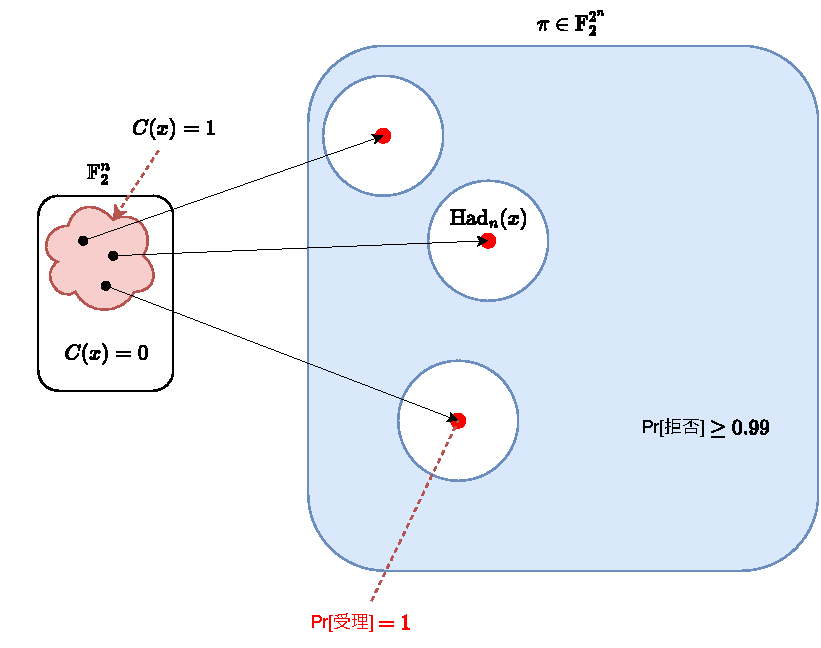
\includegraphics[width=0.8\textwidth]{images/circuit_verification.pdf}
    \caption{\cref{thm:circuit-verification}の検証者のイメージ. $C(x)=1$を満たす$x\in\F_2^n$に対し, $\pi_x=\Had_n(x)$ならば, ある$\pi\in \F_2^{2^{n^2}}$に対し, $V^{\pi_x,\pi}(C)$は確率$1$で受理する. 一方, $C(x)=1$を満たす任意の$x\in\F_2^n$に対して$\dist(\pi,\Had_n(x))\ge 0.01$を満たす任意の$\pi\in \F_2^{2^{n^2}}$に対して, $V^{\pi_x,\pi}(C)$は確率$0.99$で拒否する.}
  \end{figure}

  \begin{proof}
    入力として与えられた回路$C$に対し, \cref{thm:ThreeQuadEQ-NP-complete}で与えたカープ帰着を用いて$\QuadEQ$のインスタンス$(f_k)_{k\in [m]}$を構成する (ここで, $C$のサイズ$s$に対して$m=n+s+1$である).
    さらにこの$\QuadEQ$のインスタンス$(f_k)_{k\in[m]}$に対し, \cref{eq:M-matrix,eq:b-vector}で定義される行列$M\in\F^{m\times n^2}$とベクトル$b\in\F^m$を構成する.
    このとき, 任意の$x\in\F_2^n$に対し, 以下は同値である:
    \begin{itemize}
      \item $C(x)=1$ (ここでは$x$を$\binset^n$の元として扱う)
      \item 全ての$k\in[m]$に対し, $f_k(x)=0$
      \item $y_{i,j}:=x_i\cdot x_j$で定まるベクトル$y\in\F_2^{n^2}$は$My=b$を満たす.
    \end{itemize}
  
    以下では, 三つ目の条件を検証するPCP検証者を与える.

    \begin{algo}{}{QuadEQ-PCP}
      PCP検証者$V^{\pi_x,\pi}(M,b)$を以下で記述する:
      \begin{enumerate}
        \item 入力として$M\in\F_2^{m\times n^2}$と$b\in\F_2^m$および証明として$\pi_x\colon\F_2^n\to\F_2$と$\pi\colon\F_2^{n^2}\to\F_2$へのオラクルアクセスを受け取る.
        \item \cref{thm:linearity-test}のアルゴリズムを$\pi_x,\pi$のそれぞれに対して実行し, $\pi_x,\pi$が線形関数に$0.01$-近いかどうかを検証する. もしいずれかの実行においてこのアルゴリズムが拒否したら拒否する.
        \item \cref{lem:tensor-product-verification}の検証者を, オラクルとして$\pi_x$と$\pi$を用いて実行する. この検証者が拒否したら拒否する.
        \item \cref{lem:linear-equation-solution-verification}の検証者を, 入力として$(M,b)$, オラクルとして$\pi$を用いて実行する. この検証者が拒否したら拒否する.
        \item ここまでのステップで拒否していなければ受理して終了する.
      \end{enumerate}
    \end{algo}

    この検証者$V^{\pi_x,\pi}$が所望のPCP検証者であることを確認する.
    \cref{thm:linearity-test,thm:local-verification-LinEq,lem:tensor-product-verification,lem:linear-equation-solution-verification}ではそれぞれオラクルアクセスは$O(1)$回であり, 内部で用いるランダムビットは$O(n^2)$である.

    $C(x)=1$となるような$x\in\F_2^n$に対して$\pi_x=\Had_n(x)$であるとする.
    このとき入力$(M,b)$は, $y_{i,j}=x_i\cdot x_j$で定まるベクトル$y\in\F_2^{n^2}$に対して$My=b$を満たす.
    この$y$に対して, $\pi=\Had_{n^2}(y)$とする (補題の仮定より, $\pi_x=\Had_n(x)$である).
    このとき, 
    \begin{itemize}
      \item ステップ2では, $\pi_x,\pi$はどちらも線形関数であるため, 拒否する確率は$0$である.
      \item ステップ3では, 実際に全ての$i,j\in [n]$に対して$y_{i,j}=x_i\cdot x_j$が成り立つため, 拒否する確率は$0$である.
      \item ステップ4では, 実際に$y$は$My=b$の解であるため, 拒否する確率は$0$である.
    \end{itemize}
    以上より, $V^{\pi_x,\pi}$は確率$1$で受理する.

    次にオラクル$\pi_x$が, $C(x)=1$を満たす任意の$x\in\F_2^n$に対して$\dist(\pi_x,\Had_n(x))\ge 0.01$を満たすとする. オラクル$\pi\colon\F_2^{n^2}\to\F_2$を任意に固定する.

    \begin{itemize}
      \item $\dist(\pi,\Had_{n^2})\ge 0.01$または$\dist(\pi_x,\Had_n)\ge 0.01$ならば, 検証者はステップ2において確率$0.99$で拒否する. 以降では$\pi,\pi_x$はどちらも線形関数に十分近いとし, $\pi$に最も近い線形関数を$\Had_{n^2}(y)$とし, $\pi_x$に最も近い線形関数を$\Had_n(x)$とする. このとき, $\pi_x$の仮定から$C(x)=0$である.
      \item ステップ3は, \cref{lem:tensor-product-verification}の仮定が満たされているため, ある$i,j\in[n]$に対して$y_{i,j}\ne x_i\cdot x_j$となるならば, 確率$0.99$で拒否する.
      従って以降ではさらに$x\in\F^n,y\in\F^{n^2}$が, 全ての$i,j\in [n]$に対し$y_{i,j}=x_i\cdot x_j$を満たすとする.
      \item ステップ4は, $C(x)=0\iff My\ne b$であるため, \cref{lem:linear-equation-solution-verification}の検証者が確率$0.99$で拒否する.
    \end{itemize}
    以上より, $V^{\pi_x,\pi}$がステップ2-4のループで拒否する確率は少なくとも$0.97$である.
  \end{proof}
    
  実は\cref{thm:circuit-verification}から即座に弱いPCP定理が示せる.
  \begin{proof}[\cref{thm:weak-PCP-theorem}の証明.]
    \cref{thm:Cook-Levin}より, 回路充足可能性判定問題はNP完全である.
    従って, この問題に対するPCP検証者を与えればよい.
    実は, \cref{thm:circuit-verification}の検証者がこの条件を満たす.

    実際,
    入力として与えられた回路$C\colon\binset^n\to\binset$がYesインスタンスならば,
    ある$x\in\binset^n$が存在して$C(x)=1$となる.
    この$x$を$\F_2^n$の元とみなして, $\pi_x = \Had_n(x)$とすれば, ある$\pi$が存在して$V^{\pi_x,\pi}(C)$は確率$1$で受理する.

    一方, $C$がNoインスタンスならば, $C(x)=1$となるような$x\in\binset^n$は存在しないため, どのような$\pi_x,\pi$に対しても, $V^{\pi_x,\pi}(C)$は確率$0.99$で拒否する.    
  \end{proof}

\begin{remark}{近接PCP}{PCPP}
  \cref{thm:circuit-verification}のように, 入力として回路$C$が与えられ, さらに$C$が受け取る入力$x$を符号化したもの$\pi_x$および「追加の情報」をもつ$\pi$へのオラクルアクセスが与えられたとき, $x$が$C$の充足割り当てを符号化したものから遠い場合に高確率で拒否するような検証者は一般に充足可能性の検証よりも強いことを主張しており, これを達成するような証明のことを\emph{近接PCP} (PCP of Proximity)と呼び, 検証者のことをPCPP検証者と呼ぶ.
\end{remark}

\section{二入力回路の割り当てに対するPCP検証者}
\cref{thm:circuit-verification}はある意味で, $x\in\binset^n$を全て見ることなく, 与えられた回路$C$に対し$C(x)=1$となるかどうかを検証するPCP検証者を構成した (実際には$\pi_x=\Had_n(x)$および追加の情報$\pi_y$へのオラクルアクセスも仮定している).

ここでは回路$C$が二つの入力$x,y\in\binset^n$を受け取る場合でも同様のPCPP検証者が構成できることを示す.
この設定は人工的な問題設定に見えるが, PCP定理の証明において重要な役割を果たす.


\begin{theorem}{二入力回路の割り当てに対するPCP検証者}{two-input-circuit-PCP}
  以下を満たす定数$q=O(1)$と多項式時間乱択オラクルアルゴリズム$V^{\pi_x,\pi_y,\pi}(C)$が存在する:
  \begin{itemize}
    \item 入力として$C\colon\binset^n\times\binset^n\to\binset$および三つのオラクル$\pi_x,\pi_y, \pi$へのオラクルアクセスを受け取り, これらのオラクルに対して合計で高々$q$回のオラクルアクセスを行う.
    \item $C(x,y)=1$を満たす$x,y\in\F_2^n$に対して$\pi_x=\Had_n(x)$および$\pi_y=\Had_n(y)$であるならば, ある$\pi\in \F_2^{2^{2n} + 2^{4n^2}}$が存在して, $V^{\pi_x,\pi_y,\pi}(C)$は確率$1$で受理する.
    \item $C(x,y)=1$を満たす任意の$x,y\in\F_2^n$に対して$\dist(\pi_x,\Had_n(x))\ge0.01$または$\dist(\pi_y,\Had_n(y))\ge0.01$を満たす任意の$\pi_x,\pi_y$および任意の$\pi$に対して, $V^{\pi_x,\pi_y,\pi}(C)$は確率$0.99$で拒否する.
  \end{itemize}
\end{theorem}

$(x,y)$を一つの文字列$z\in\F_2^{2n}$とみなして\cref{thm:circuit-verification}を適用したとき, 検証者は$\pi_z=\Had_{2n}(z)$と追加の情報$\pi$へのオラクルアクセスを持つことになるが,
\cref{thm:two-input-circuit-PCP}の検証者は, $x,y$それぞれの符号化$\pi_x,\pi_y$へのオラクルを持つという点が異なっている.

\cref{thm:two-input-circuit-PCP}の証明においては, ある文字列$x\in\binset^n$が別の文字$\overline{x}\in\binset^{n+m}$の接頭辞かどうかを(オラクルアクセスを用いて)局所的に検証することを意味する以下の補題を用いる.
\begin{lemma}{接頭辞の検証}{concatenation-test}
  以下を満たす定数$q=O(1)$と多項式時間乱択オラクルアルゴリズム$V_0^{\pi_x,\pi_{\overline{x}}}(1^n,1^m)$が存在する:
  \begin{itemize}
    \item オラクル$\pi_x,\pi_{\overline{x}}$は, ある$x\in\F_2^n$と$\overline{x}\in\F_2^{n+m}$に対して, $\dist(\pi_x,\Had_n(x))<0.01$および$\dist(\pi_{\overline{x}},\Had_{n+m}(\overline{x}))<0.01$であることが保証されている.
    \item 検証者$V_0^{\pi_x,\pi_{\overline{x}}}$は高々$q$回のオラクルアクセスを行う.
    \item $\pi_x = \Had_n(x)$, $\pi_{\overline{x}}=\Had_{n+m}(\overline{x})$であって, さらに$\overline{x}$の先頭$n$文字が$x$と一致するならば, $V_0^{\pi_x,\pi_{\overline{x}}}$は確率$1$で受理する.
    \item 一方, $\overline{x}$の先頭$n$文字が$x$に一致しない場合, 確率$0.99$で拒否する.
  \end{itemize}
\end{lemma}
\begin{proof}
  アルゴリズム$V_0^{\pi_x,\pi_{\overline{x}}}$は単純で, 以下のように記述できる:
  \begin{enumerate}
    \item 一様ランダムなベクトル$r\sim\F_2^n$を選び, $\overline{r}=(r,0^m)\in\F_2^{n+m}$とする.
    \item $\pi_x(r) \ne \pi_{\overline{x}}(\overline{r})$ならば拒否する. ここで, $\pi_{\overline{x}}(\overline{r})$は\cref{lem:nearest-linear-function-evaluation}を用いて計算する.
    \item ステップ1-2を10回繰り返し, 一度も拒否しなければ受理して終了する.
  \end{enumerate}

  $\overline{x}$の最初の$n$文字を$y\in\binset^n$とする.
  もしも$\pi_x=\Had_n(x)$, $\pi_{\overline{x}}=\Had_{n+m}(\overline{x})$であって, $y=x$ならば, ステップ2においてどのような$r\sim\F_2^n$を選んでも$\Had_n(x)(r) = \Had_n(y)(r) = \Had_{n+m}(\overline{x})(r,0^m)$となり, 確率$1$でアルゴリズムは受理する.
  一方で$x\ne y$の場合を考える. オラクル$\pi_{\overline{x}}$は$\Had(\overline{x})$に$0.01$-近いため,
  \cref{lem:nearest-linear-function-evaluation}より, ステップ2において, 確率$0.98$で$\pi_{\overline{x}}(\overline{x})=\Had_n(y)(r)$を計算できる. また, $r$が一様ランダムなので, 確率$0.99$で$\pi_x(r)=\Had_n(x)(r)$である.
  従って一度の試行で少なくとも確率$0.97$で検証者は拒否するため,
  ステップ1-2を10回だけ繰り返せば少なくとも確率$0.99$で検証者は拒否する.
\end{proof}

\begin{remark}{接尾辞の検証}{suffix-test}
  \cref{lem:concatenation-test}のアルゴリズムは$x$が$\overline{x}$の接頭辞かどうかの検証を行うが, 同様のアルゴリズム ($0^m$と$r$の順番を反転させるだけ)を考えれば接尾辞の検証にも利用できる.
\end{remark}

\begin{proof}[\cref{thm:two-input-circuit-PCP}の証明.]
三つ目のオラクル$\pi\in\binset^{2^{2n} + 2^{4n^2}}$を, 以下の二つの関数の組として解釈する:
\begin{itemize}
  \item $\pi_1 \colon \F_2^{2n} \to \F_2$. この関数は, ベクトル$\overline{x}:=(x,x')\in\F_2^{2n}$に対して$\pi_1 = \Had_{2n}(\overline{x})$であることを想定する.
  \item $\pi_2 \colon \F_2^{4n^2} \to \F_2$. この関数は, 上記のベクトル$\overline{x}$に対し$\overline{y}_{i,j} = \overline{x}_i\cdot \overline{x}_j$で定まるベクトル$\overline{y}\in\F_2^{4n^2}$に対し, $\pi_2 = \Had_{4n^2}(\overline{y})$であることを想定する.
\end{itemize}
なお, 実際には$\pi_1,\pi_2$は関数としては解釈できるが, その関数が線形関数であるとは限らない.
\cref{alg:QuadEQ-PCP}を少し修正した以下の検証者$V^{\pi_x,\pi_{y},\pi}(C)$を考える:

\begin{algo}{}{two-input-circuit-PCP}
  PCP検証者$V^{\pi_x,\pi_{y},\pi}(C)$を以下で記述する:
  \begin{enumerate}
    \item オラクル$\pi$を二つの関数$\pi_1\colon\F_2^{2n}\to\F_2,\pi_2\colon\F_2^{4n^2}\to\F_2$の組として解釈する.
    \item 入力で与えられた回路を$C\colon\binset^{2n}\to\binset$とみなし, \cref{thm:circuit-verification}の証明で考えた行列$M\in\F_2^{m\times {(2n)^2}}$とベクトル$b\in\F_2^m$を計算する.
    \item \cref{thm:linearity-test}のアルゴリズムを$\pi_x,\pi_y,\pi_1,\pi_2$に対して実行し, $\pi_1,\pi_2$がそれぞれ線形関数に$0.01$-近いかどうかを検証する. もしいずれかの実行においてこのアルゴリズムが拒否したら拒否する.
    \item $\pi_x,\pi_y,\pi_1$に最も近い線形関数をそれぞれ$\Had_n(x),\Had_n(y),\Had_{2n}(z)$とする.
    \item $z\in\F_2^{2n}$の前半の$n$文字が$x$, 後半の$n$文字が$y$に一致するかどうかをそれぞれ\cref{lem:concatenation-test}のアルゴリズムを用いて検証する. もしいずれかの検証においてこのアルゴリズムが拒否したら拒否する.
    \item \cref{lem:tensor-product-verification}の検証者を, オラクルとして$\pi_1$と$\pi_2$を用いて実行する. この検証者が拒否したら拒否する.
    \item \cref{lem:linear-equation-solution-verification}の検証者を, 入力として$(M,b)$, オラクルとして$\pi_2$を用いて実行する. この検証者が拒否したら拒否する.
    \item ここまでのステップで拒否していなければ受理して終了する.
  \end{enumerate}
\end{algo}

$C(x,y)=1$を満たす$x,y\in\F_2^n$に対し$\pi_x=\Had_n(x)$, $\pi_y=\Had_n(y)$とする.
このとき, 文字列$x,y$を結合して得られる文字列を$z=(x,y)\in\F_2^{2n}$,
また文字列$w\in\F_2^{4n^2}$を, $w_{i,j}=z_i\cdot z_j$と定めると,
$V^{\Had_n(x),\Had_n(y),\Had_{2n}(z),\Had_{4n^2}(w)}(C)$は確率$1$で受理する.

一方, オラクル$\pi_x,\pi_y$が, $C(x,y)=1$を満たす任意の$x,y\in\F_2^n$に対して, $\dist(\pi_x,\Had_n(x))\ge 0.01$または$\dist(\pi_y,\Had_n(y))\ge0.01$の少なくとも一方が成り立つとする.
任意にオラクル$\pi_1,\pi_2$を固定する.
\begin{itemize}
  \item ステップ3では全てのオラクルが線形関数に近いかどうかを確認しており, もしもどれかが線形関数から$0.01$-遠いならば, \cref{thm:linearity-test}より確率$0.99$で検証者は拒否する. それぞれに最も近い文字列を$x\in\F_2^n,y\in\F_2^n,z\in\F_2^{2n}$とする.
  \item ステップ4では$z=(x,y)$かどうかが確認される. もしも$z\ne(x,y)$ならば確率$0.99$で拒否される.
  \item ステップ5以降は\cref{thm:circuit-verification}と同一であり, 特に$\pi_1$が$C$の任意の充足割り当てから$0.01$-遠い場合は確率$0.99$で検証者は拒否する. さらにこのとき, 任意の充足割り当て$(x^*,y^*)\in C^{-1}(1)$に対して, $\dist(x,x^*)\ge0.01$もしくは$\dist(y,y^*)\ge 0.01$が成り立つ (\cref{exer:split-vector-distance}).
\end{itemize}
\end{proof}

\begin{exercise}{二つに分割したベクトルの距離}{split-vector-distance}
  ベクトル$z\in\F_2^{2n}$に対し, その前半$n$個の成分からなる部分ベクトルを$\mathrm{head}(z)\in\F_2^n$, 後半$n$個の成分からなる部分ベクトルを$\mathrm{tail}(z)\in\F_2^n$とする.
  集合$S\subseteq\F_2^{2n}$を任意に固定する.
  もしもベクトル$z$が$\dist(z,S)\ge \epsilon$, すなわち, 任意の$s\in S$に対して$\dist(z,s)\ge \epsilon$を満たすならば,
  任意の$s\in S$に対して
  \begin{itemize}
  \item $\dist(\mathrm{head}(z),\mathrm{head}(s))\ge \epsilon$
  \item $\dist(\mathrm{tail}(z),\mathrm{tail}(s))\ge \epsilon$
  \end{itemize}
  の少なくとも一方が成り立つことを示せ.
\end{exercise}